\documentclass{article}

% \usepackage{icml2023}
\usepackage[accepted]{icml2023}

% Packages
\usepackage{hyperref}
\usepackage{graphicx}
\usepackage{booktabs}
\usepackage{multirow}
\usepackage{amsmath}

% Running Title
\icmltitlerunning{DiLoCo-SWARM}

\begin{document}

% Title
\twocolumn[
  \icmltitle{DiLoCo-SWARM: Early Steps Towards Scalable Decentral Learning}
  \begin{icmlauthorlist}
    \icmlauthor{Mika Senghaas}{epfl}
  \end{icmlauthorlist}
  \icmlaffiliation{epfl}{EPFL}
  \icmlkeywords{Distributed Training, Decentralized AI, SWARM, DiLoCo}
  \vskip 0.3in
]

% Abstract
\begin{abstract}
  ...
\end{abstract}

\section{Introduction}

% Centralized training
Modern foundation models have billions of parameters and are trained on
trillions of tokens~\cite{kaplan2020,hoffmann2022,brown2023}. Operating at such
scale requires orchestrating thousands of GPUs to distribute
computation~\cite{dubey2024,deepseekai2024}. However, traditional
parallelization techniques, such as data and pipeline parallelism, rely on fast
interconnect to not significantly bottleneck training. Hence, frontier-scale
models can currently only be trained in highly-specialized data centers.
Operating such data centers requires multi-million, sometimes billions of
dollars, and, as a result, research capabilities are increasingly confined to a
small number of corporate and state entities, creating significant points of
control, increased risk of capability capture or misue~\cite{intellect1}.

% Prime on centralization
% The current trajectory of AI development shows increasing consolidation of
% computational resources and research capabilities to a small number of corporate
% and state entities. As the cost of training competitive frontier models
% increases, this consolidation only accelerates. While centralization has the
% benefit of reduced coordination costs, and increased efficiency, it has the
% negative externality of creating significant points of control and increased
% risk of capability capture or misuse.

% Decentralized training
Recently, decentralized training has emerged as a promising counter-weight. It
is based on the idea of pooling the vast, cheap compute resources across the
globe for collaborative model training. It promises smaller entitires access to
large-scale compute at significantly reduced cost, with the potential to
accelerate open-source AI development and research. However, this new paradigm
comes with significant technical and algorithmic challenges: nodes have to
communicate via common internet connections, leading to orders of magnitude
lower network bandwidths compared to common HPC environments, and the pool of
training nodes can be heterogeneous and dynamic, with nodes joining or leaving
the training unpredictabtly. 

% Prime on decentralization
% However, there is increasing interest in enabling training across geographically
% distributed nodes, leveraging standard internet connections to pool GPU
% resources for collaborative model training. This paradigm shift introduces new
% challenges: network bandwidth between nodes can be up to three orders of
% magnitude lower than in typical HPC environments, and the pool of training nodes
% can be dynamic, with nodes joining or leaving the process unpredictably, making
% system reliability a critical concern

% Prime on implications of INTELLECT-1
% The successful training of INTELLECT-1 demonstrates a key technical advancement
% in enabling a more open and decentralized AI ecosystem, with significant
% implications for the future development and governance of advanced artificial
% intelligence systems.  The current trajectory of AI development shows increasing
% consolidation of computational resources and research capabilities to a small
% number of corporate and state entities. As the cost of training competitive
% frontier models increases, this consolidation only accelerates. While
% centralization has the benefit of reduced coordination costs, and increased
% efficiency, it has the negative externality of creating significant points of
% control and increased risk of capability capture or misuse.  Open-source AI
% currently serves as the best counterweight to a closed-source AI ecosystem, and
% has yielded significant advancements in virtually every technical aspect of
% artificial intelligence development. However, open-source AI has yet to amass
% the scale of compute that is relevant to achieve parity with the largest
% closed-source AI labs. This is a requirement if the open-source ecosystem
% intends to train and open-source competitive frontier models. As demonstrated by
% this work and prior results on collaborative deep learning (Pascutto and
% Linscott, 2019; Diskin et al., 2021; Borzunov et al., 2022), decentralized
% training has the potential to enable that scale of compute by making it possible
% to pool resources across the world for training large-scale foundational models.
% Historical precedent from distributed compute protocols and incentive networks
% demonstrates the potential scale of community-pooled compute resources.
% Bitcoin’s network grew from a few personal computers to over 10 Gigawatts of
% compute in 12 years, and Ethereum’s network reached similar scale before
% transitioning to proof of stake. These networks demonstrate how properly aligned
% economic incentives can mobilize massive computational resources across
% geographical and institutional boundaries. Similar dynamics could emerge in
% decentralized AI training: with appropriate incentive mechanisms and technical
% infrastructure, community-pooled AI training could potentially exceed the
% compute capacity of any centralized training facilities.

% Intellect-1 and DiLoCo
Hence, currently decentral training efforts can not yet match the scale and
efficiency of the centralized setting, but the pace of research and advancements
in the field has picked up significantly. INTELLECT-1~\cite{intellect1}, a 10B
parameter model trained across three continents, is the most recent
demonstration that large-scale decentral model training is possible. The model
is a scale-up of DiLoCo~\cite{douillard2023}, a low-cost communication
distributed data parallel (DDP) training method. Compared to traditional DDP,
DiLoCo's key insight is to replace regular gradient synchronization at every
step with less frequent synchronization using an inner-outer optimization
scheme. Their empirical results show that the method maintains performance while
requiring a fraction of the communication cost, i.e. only every 500 steps.  The
experiments have since been replicated, and scaled to billion-parameter through
engineering advances in the fault tolerance of the
algorithm~\cite{jaghouar2024,intellect1}, making it a state-of-the-art method
for decentralized training. However, a key limitation is that each node has to
store a full copy of the model to participate during training. For example, to
train the 10B INTELLECT-1, the minimum requirement for a single node were 8xH100
GPUs.

% SWARM
SWARM~\cite{ryabinin2023} parallelism is a promising, but less explored,
alternative for decentralized training that is designed from the ground-up for
larger scale. Unlike DiLoCo, which relies solely on data parallelism, SWARM
combines data and pipeline parallelism. By also sharding the model, SWARM has
the potential to scale to larger models, or vice versa, allow lower-end devices
to participate in training, making it an attractive candidate for further
scaling decentralized training efforts. In its original formulation, SWARM
requires gradient synchronization between all nodes serving the same pipeline
stage of a model.

% DiLoCo-SWARM
The above motivates this work which makes the following two main contributions:

% Implementation

\begin{enumerate}
  \item \textbf{DiLoCo-SWARM.} We show that SWARM parallelism is compatible with
  DiLoCo-style gradient synchronization, allowing to train SWARM while requiring 
  significantly fewer synchronization of gradients without sacrificing performance.
  \item \textbf{Implementation.} We release a re-implementation
  of a feature subset of SWARM parallelism. Instead of multiple thousands, the
  implementation uses a few hundred lines of pure PyTorch code.
\end{enumerate}

Besides open-sourcing the full experiment code and results on
\href{https://github.com/mikasenghaas/swarm}{GitHub} and
\href{https://wandb.ai/mikasenghaas/swarm}{Weights \& Biases}, we release the
distilled version of the minimal SWARM re-implementation as a
\href{https://gist.github.com/mikasenghaas/5fa1aa77ea69f187f531a5889983c249}{GitHub
Gist}. We hope that these resources can act as a starting point for furter
open-source efforts in this domain to scale SWARM, and other decentralized
training methods, from research to production-grade systems to make decentral AI
reality.

\section{Background}

\subsection{Distributed Training}

In distributed training, $n$ nodes collaboratively train a \textit{model},
represented as a set of parameters $\theta$, on a \textit{dataset}, represented
as a set of samples $D = \{(\mathbf{x}_e, \mathbf{y}_1),\dots\}$. Collaboration 
means that each node runs part of the computation, and occasionally communicates
intermediate results. Two of the most commonly used forms of distributing
computation are data and model parallelism.

\begin{figure}[h]
    \centering
    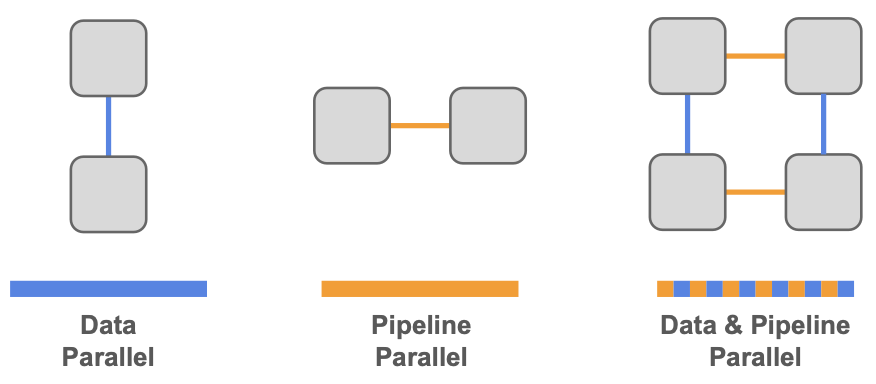
\includegraphics[width=0.45\textwidth]{figures/parallelization.png}
    \caption{}
    \label{fig:parallelization}
\end{figure}

\textit{Data parallelism} partitions the dataset, creating $n$ data shards
$D_1,\dots,D_n$. The $i$-th node only holds a (local) data shard $D_i$ and a
copy of the full model parameters $\theta$. Training proceeds as shown in
Algorithm X: Each node samples a batch from its local data shard,
computes local gradients via a full forward and backward pass, but before
updating the model, averages the gradients from all workers, typically via an
AllReduce. The only communication pattern, which we will denote simply as DP
communication, is the AllReduce operation. Its cost scales with the number
of model parameters $|\theta|$ and number of nodes $n$.

\begin{algorithm}
\caption{Data Parallel Gradient Synchronization}
\label{alg:dp}
\begin{algorithmic}
\STATE {\bfseries Input:} Local Dataset $D_i$, Model $\theta^{(t-1)}$, Optimizer $\mathtt{OPT}$, Loss $\mathcal{L}$
\STATE Sample batch: $x_i\sim D_i$
\STATE Compute gradient: $g_i \gets \nabla_{\theta_i} \mathcal{L}(x_i; \theta^{(t-1)})$
\STATE Sync gradients: $g \gets \frac{1}{n}\sum_{i}^n g_i$ \COMMENT{$\mathtt{AllReduce}$}
\STATE Update model: $\theta_i^{(t)} \gets \mathtt{OPT}(\theta_i^{(t-1)}, g)$
\end{algorithmic}
\end{algorithm}

\textit{Pipeline parallelism} partitions the model, creating $n$ sequential
model shards, $\theta=\theta_1\circ\dots\circ\theta_n$. Due to their sequential
dependency, the shards are said to represent a "stage" of the pipeline, where
the $i$-th stage serves the model shared $\theta_i$. For most deep learning
model such a sequential partition is very natural, as they are architected as
repeated computational blocks. For example, in modern LLMs one stage handles one
or more Transformer blocks. The partitioning creates a bi-directional
communication pattern between stages during training, which we refer to as PP
communication: During a forward pass activations are communicated from stage $i$
to $i+1$, and during the backward pass gradients are sent from stage $i$ to
$i-1$.  Despite its simplicity, pipeline parallelism is notoriously hard to make
efficient. Naive implementations suffer from significant GPU idle time, e.g.
when the first node has to wait for the full pipeline forward and backward pass
before updating the first model shard. Efficient pipeline parallel
implementation therefore rely on micro-batching and advanced scheduling
techniques to be practically viable. Generally speaking, PP communication scales
with the number of stages $n$ and the model's hidden dimension.

\textit{2D parallelism} Data and pipeline parallelism can be combined, which is
sometimes referred to as 2D parallelism. Here, nodes are arranged in a $m\times
n$ grid, where each node handles data shard $D_i$ and model shard $\theta_j$.
The DP and PP communication patterns are interleaved. Local gradients are
computed using PP communication by forwarding and backward passes through the
pipeline stages for each data shard individually. Then, to update the model
shards, an \texttt{AllReduce} operations runs to average gradients within each
stage.

\subsection{DiLoCo}

% DiLoCo
In the decentralized setting, interconnect may be slow and so regular gradient
synchronization as shown in Algorithm X can bottleneck the training process,
especially when scaling to larger models. DiLoCo~\cite{douillard2023} is a
low-communication data parallel training method that reduces the frequency at
which gradients are synchronized. DiLoCO proposes a dual optimization scheme.
As shown in Algorithm Y each node trains for a fixed number of inner steps $H$
using a local optimizer. To synchronize with the remaining workers, it computes
a pseudo-gradient as the difference between the parameters before and after the
inner optimization. The pseudo-gradients are then averaged between all nodes via
\texttt{AllReduce} and a global model is updated using an outer optimizer. 

\begin{algorithm}
\caption{DiLoCo Gradient Synchronization}
\label{alg:diloco}
\begin{algorithmic}[1]
\STATE \textbf{Input:} Local dataset $D_i$, Model $\theta^{(t-1)}$, Optimizers $\mathtt{OPT}_{\text{local}}$ and $\mathtt{OPT}_{\text{global}}$, Loss $\mathcal{L}$, Local Steps $H$ 
\STATE Copy global model: $\theta_i^{(t-1)} \gets \theta^{(t-1)}$
\FOR{$H$ steps}
  \STATE Sample batch: $x \sim D_i$
  \STATE Compute gradient: $g_i \gets \nabla_{\theta_i} \mathcal{L}(x_i; \theta_i^{(t-1)})$
  \STATE Update local model: $\theta_i^{(t-1)} \gets \mathtt{OPT}_{\text{local}}(\theta_i^{(t-1)}, g_i)$
\ENDFOR
\STATE Compute pseudo-gradient: $\Delta_i \gets \theta_i^{(t-1)} - \theta^{(t-1)}$
\STATE Sync pseudo-gradients: $\Delta \gets \frac{1}{n}\sum_i^n \Delta_i$ \COMMENT{$\mathtt{AllReduce}$}
\STATE Update global model: $\theta^{(t)} \gets \mathtt{OPT}_{\text{global}}(\theta^{(t-1)}, \Delta)$
\end{algorithmic}
\end{algorithm}

\subsection{SWARM}

% SWARM
Pipeline parallelism presents itself as a natural solution. However, traditional
pipeline parallelism struggles with heterogeneous workers and node failures. Due
to its inherently sequential nature, the pipeline is bottlenecked by its weakest
link, leading to idle time for quicker workers. Furthermore, a single node
failure will stall the entire training procedure, rendering the algorithm not
fault-tolerant.

SWARM parallelism~\cite{ryabinin2023} addresses these issues and proposes a
decentralized training method combining data and pipeline parallelism. Instead
of organizing nodes in a rigid two-dimensional grid of deterministic pipelines,
SWARM constructs a stochastic pipeline on-the-fly: Here, activations are
forwarded stochastically based on statistical estimates on the throughput of
adjacent peers. This ensures that faster or better-connected nodes receive more
requests and sit less idle. Once all micro batches are processed by SWARM, local
gradients of models shards are synchronized within pipeline stages using regular
gradient synchronization every step.  SWARM is designed from the ground up to be
fault-tolerant. Forward or backward requests which are not fulfilled within some
timeout, are re-routed to other peers. Further, nodes periodically switching
from under- to overutilised stages to distribute workload.

% Key observation: Square-cube law

Empirical results show that SWARM 

Unlike DiLoCo, SWARM naturally scales to larger models and handles heterogenity
in the worker pool. However, even with advanced pipelining schedules, there are 
sequential dependencies between workers, creates communication overhead which 
reduces compute utilization compared to DiLoCo, where nodes train truly
independent locally between global synchronization.

\section{DiLoCo-SWARM}

Similarly to DDP, SWARM workers have to synchronize gradients of their model
shard during every training step within their pipeline stage. The empirical
evidence on the robustness of DiLoCo-style gradient sychronization naturally
leads to DiLoCo-SWARM, an extension of SWARM parallelism that replaces naive
gradient synchronization at every step with an inner-outer optimization that
runs periodically.

\begin{figure}[h]
    \centering
    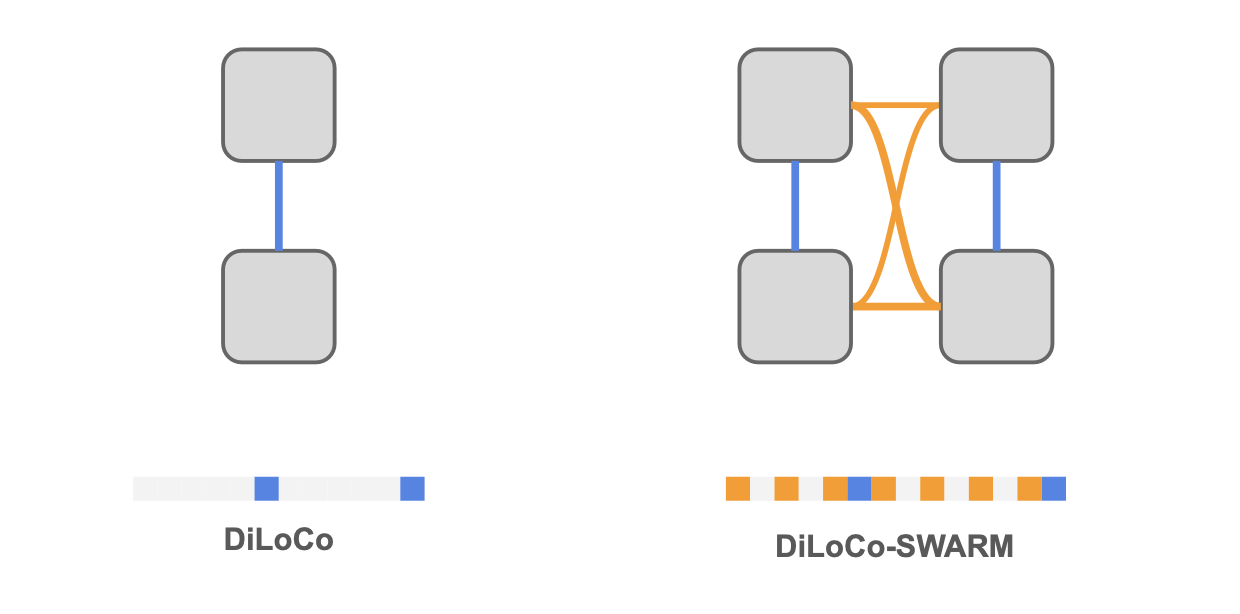
\includegraphics[width=0.45\textwidth]{figures/diloco-swarm.png}
    \caption{}
    \label{fig:diloco-swarm}
\end{figure}

\section{Implementation}

A key contribution of this work is the release of a minimal distributed training
script. Depending of its parameterization, it runs a multi-node training job
using data parallelism, tensor parallelism, or a SWARM-style combination of the
two. By optinally specifying an outer optimizer, the script replaces regular
step-wise gradient synchronization with the DiLoCo-style inner-outer
optimization scheme.

% Advantages
The implementation is designed for simplicity and readability. Instead of the
multiple thousand lines of code in the original implementation, it uses only a
few hundreds with the only dependency being PyTorch. This makes it easy for
anybody with some experience in distributed training to grasp the core ideas and
interaction being various traditional parallelization techniques, and 
state-of-the-art methods, like DiLoCo and SWARM. For small-scale testing, it can
emulate training via threads, allowing for debugging and testing without dozens
of GPUs. Because it natively integrates various parallelization techniques, and
interfaces with HuggingFace for models and datasets, it is the ideal starting
point for quickly verifying research ideas and conducting, as showcased in
DiLoCo-SWARM.

% Limitations (Not feature-complete and less efficienty)
However, as of this point, the re-implementation is not feature-complete. Due to
limitations to PyTorch distributed, it does not yet support dynamic world sizes,
over-the-internet connections, and the SWARM's fault tolerance mechanism such as
re-wiring requests. Therefore, the script can only run distributed application
on single node. While this seems to be miss the point of SWARM parallelism, it
still allows for interesting research regarding the core logic of the system. It
should also be noted that the training script does not match the efficiency
reported in the original paper which uses custom distributed communication and
storage primitives, advanced scheduling, and, whenever possible, overlaps
computation asynchronously, resulting in larger hardware utilization.

% TODO: Show in the Appendix which features are supported and which are not

% NanoGPT
The implementation should therefore be seen as a supplemental resource, which
puts emphasize on understandability, and hackability. Our hope is that it might
have a similar effect of NanoGPT, which now serves as an easy-to-hack and verify
testing ground for novel research within the open-source community.

% Implementation details
For more details on the implementation, design decision and some hacks to
circumvent limitations of PyTorch's distributed package, find more details in
the \href{https://github.com/mikasenghaas/swarm}{GitHub} repository.

\section{Experiments}

% Introduction
In this section we report the experiments validating DiLoCo-SWARM. The experiment
mostly follows the setup and hyper-parameters of DiLoCo~\cite{douillard2023}.

% Dataset
We consider a language modeling task on the FineWeb-Edu~\cite{penedo2024}
dataset, a large pre-training dataset consisting of high-quality web pages
filtered for educational content. We choose this dataset over other common
pre-training datasets due to its high token efficiency allowing to match the
original GPT-2~\cite{radford2019} performance on the
HellaSwag~\cite{zellers2019} benchmark when training the same model with 10x
less data~\cite{karpathy2024}.

% Model and 
Unless otherwise stated, we use a randomly initialized GPT-2 small as our base
model with a total of $\sim$180M parameters. Note, that this is slightly larger
than the original GPT-2 model, as we do not share the parameters of the embedding
matrix and language modeling head.

% Hyper-parameters
Training hyper-parameters are identical to those in DiLoCo~\cite{douillard2023}.
The base optimizer is AdamW with a learning rate of $4\cdot 10^{-4}$, and a
weight decay of $0.01$ which is linearly warmed up. When DiLoCo-style gradient
synchronization applies, we use a Nesterov with a learning rate of $0.7$ and a
momentum of $0.9$ as an outer optimizer. A detailed description of the
hyperparameters is provided in Table~\ref{tab:hyperparameters} in the Appendix.

% Evaluation
Our main evaluation metric is the perplexity on a held-out validation set of 10M
randomly sampled tokens. We evaluate throughout training to show the convergence
against the number of training steps.

% Main Experiment: DiLoCo-SWARM
\textbf{Main Experiment.} Our main experiment setup closely follows that of
DiLoCo~\cite{douillard2023}. We train two baselines and a DiLoCo-SWARM. The
\textit{weak baseline} trains for 2,000 steps on one GPU with a batch size of
512 and sequence length of 1024, for a total training budget of 1B tokens. The 
strong baseline is a 4x2 SWARM, i.e. eight workers distributed in two pipeline 
stages. This baseline performs regular all-reduce gradient synchronization at
every step. The higher compute budget is used to scale the batch size to the
number of worker per stage, leading to a total training budget of 4B tokens.
Finally, we train a 4x2 DiLoCo-SWARM which uses the same setup and compute
budget as the strong baseline but performs the outer optimization step only
every 50 steps.

\begin{figure}[ht]
  \centering
  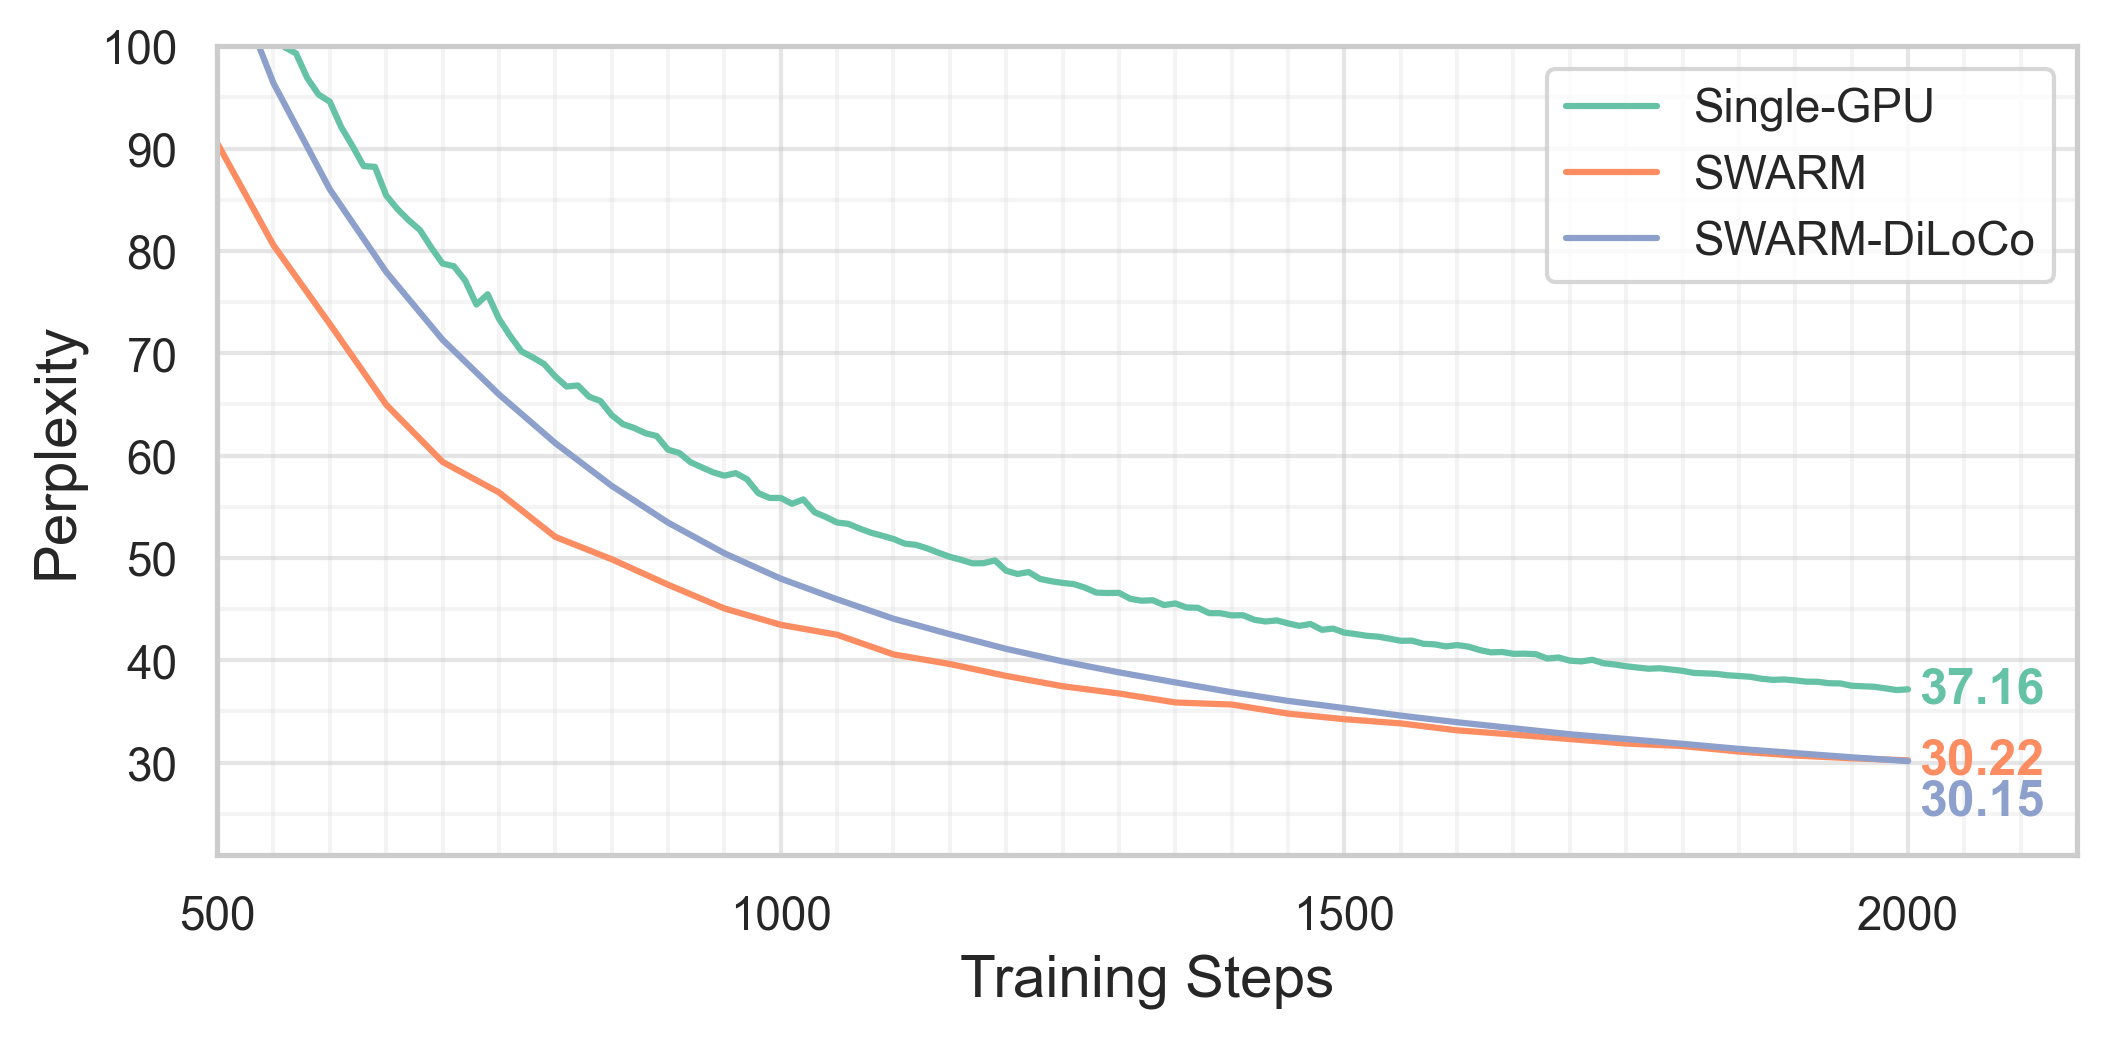
\includegraphics[width=0.45\textwidth]{figures/experiment1.png}
  \caption{\textbf{Main Result} We show the validation perplexity against the number of training steps for two baselines and SWARM-DiLoCo. With the same compute and
  data budget but with 50x less gradient synchronization, DiLoCo-SWARM matches the 
  generalization performance of the strong SWARM baselines.}
  \label{fig:experiment1}
\end{figure}

Figure~\ref{fig:experiment1} shows the validation perplexity as a function of
the training steps. Unsurprisingly, the weaker baseline, using less compute and
data, is outperformed by the stronger SWARM baseline with final perplexities of 
37.16 and 30.22, respectively. Our main finding is that DiLoCo-SWARM closely
matches, and even exceeds, the strong baseline in generalization performance
with a validation perplexity of 30.15, despite synchronizing gradients 50x fewer
times. This implies that DiLoCo-style gradient synchronization is compatible
with SWARM parallelism, allowing to reduce the communication cost incurred by 
gradient synchronization within pipeline stages of SWARM.

% Experiment 2: Ablation on communication frequency
\textbf{Communication Frequency.} We are interested in how \textit{infrequently}
gradient synchronization can occur without impacting convergence. Intuitively,
the slower the frequency, the worse convergence, but whether synchronizing every
10 or 200 steps negatively impacts performance, has implications on the
practical usefulness of the algorithm. To investigate this question we train
five models using the same training setup and only vary the number of local
training steps before performing an outer optimization step.

% TODO: Add perplexities in legend
\begin{figure}[ht]
  \centering
  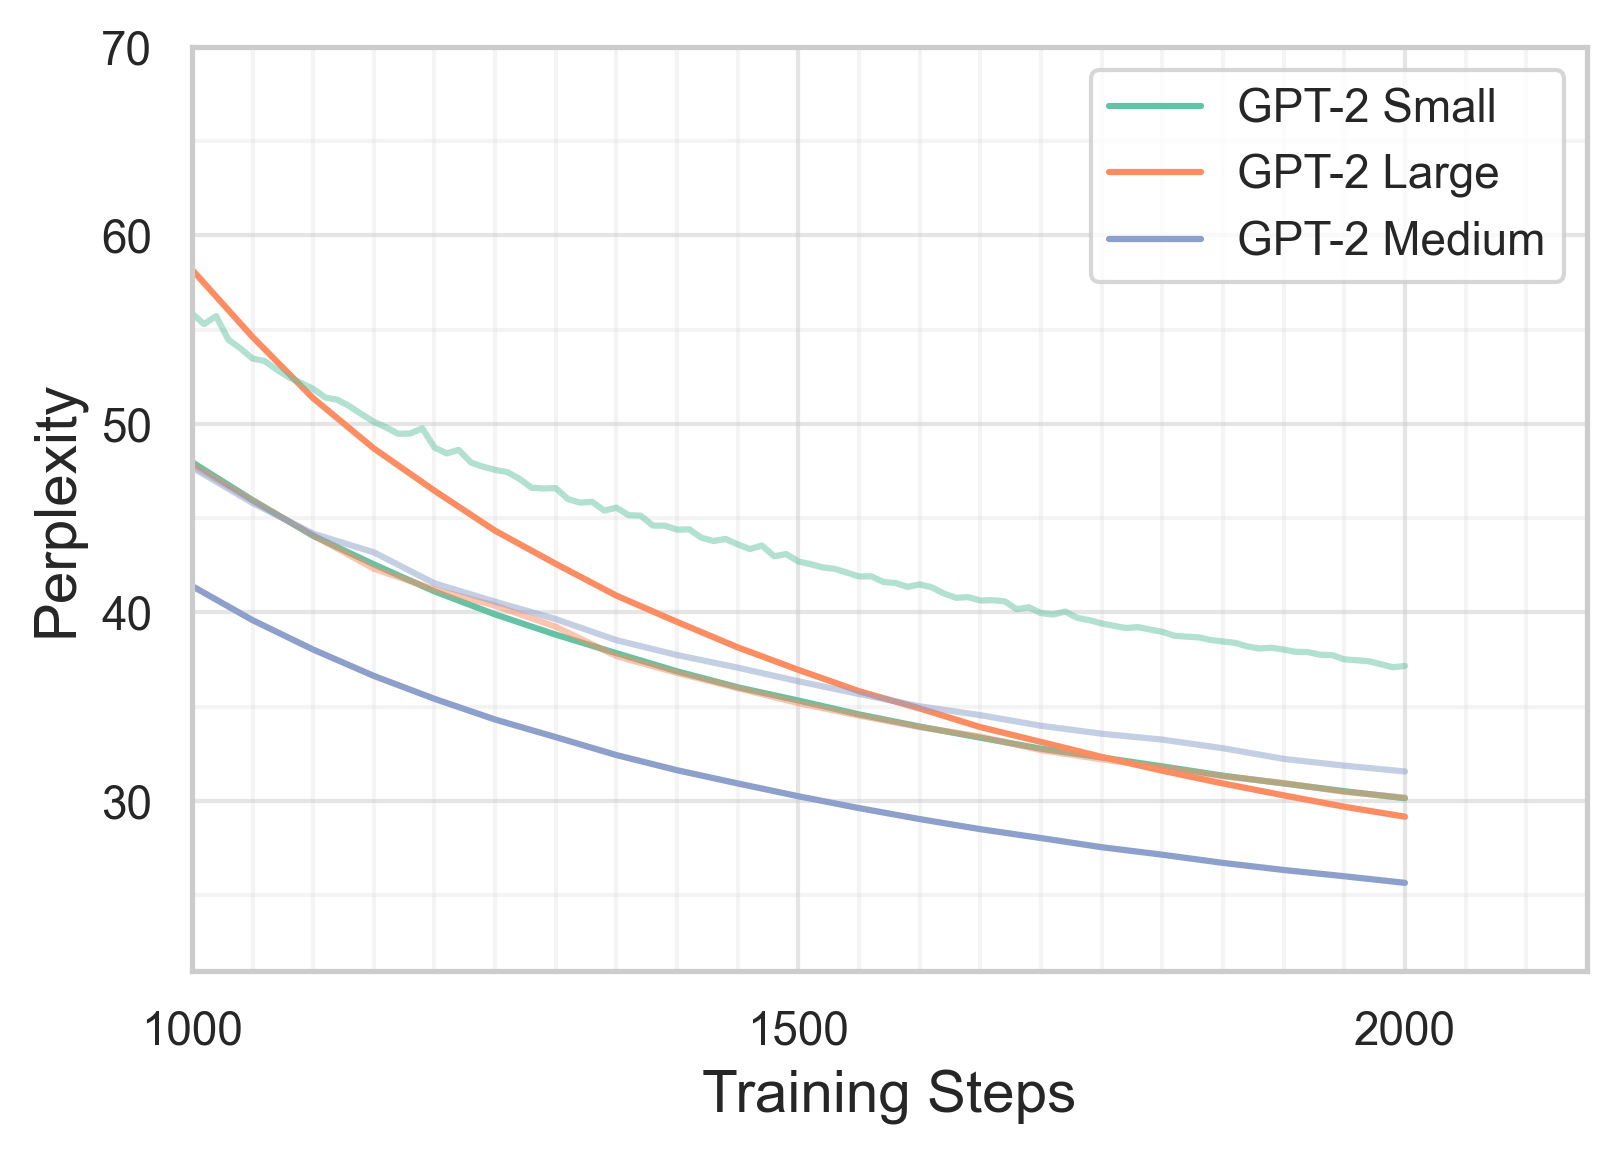
\includegraphics[width=0.45\textwidth]{figures/experiment3.png}
  \caption{\textbf{Communication Frequency} We vary the number of local training
  steps before performing an outer optimization step from $\{10, 20, 50, 100, 200\}$ 
  and report the validation perplexity throughout training. Synchronizing more
  frequently yields better results but performance degradation is neglibible even
  on all tested values.}
  \label{fig:experiment2}
\end{figure}

Figure~\ref{fig:experiment2} shows the results of this experiment. In line with
the original DiLoCo results, generalization performance monotonically increases
with higher gradient synchronization frequency. However, the performance
degradation for less frequent gradient synchronization is mild. As outlined in
Table~\ref{tab:experiment2}, synchronizing every 10 steps achieves a strong
validation perplexity of 27.95. Note, that this also significantly improves the
step-synchronous SWARM baseline in Figure~\ref{fig:experiment1} while still
reducing the synchronization frequency by 10x. In our experiments, a good
trade-off between communication frequency and performance is achieved when
synchronizing every 50 steps, which is therefore used throughout all other
experiments.

\begin{table}[ht]
\centering
\begin{tabular}{lccc}
\toprule
\textbf{Freq.} & \textbf{PPL} & \textbf{$\Delta$ (Abs./Rel.)} \\ 
\midrule
10 & 27.95 & - \\
20 & 28.61 & 0.66 / 2.36\% \\
50 & 30.15 & 2.2 / 7.87\% \\
100 & 30.49 & 2.54 / 9.09\% \\
200 & 31.27 & 3.32 / 11.88\% \\
\bottomrule
\end{tabular}
\caption{\textbf{Communication Frequency} We report the final validation
perplexity for different communication frequencies and their absolute and
relative changes compared to synchronizing every 10 steps.}
\label{tab:experiment2}
\end{table}

% Experiment 3: Varying the model size
Finally, we train different model sizes to check whether the DiLoCo-style
gradient synchronization is robust to model sizes. We use the same setup as the
main experiment but vary the number of layers, heads, and embedding dimensions,
to obtain three different GPT-2 style models. In addition to GPT-2 Small (180M
parameters), we also train GPT-2 Tiny and GPT-2 Medium, with 14M and 405M
parameters respectively.

\begin{table}[ht]
\centering
\begin{tabular}{lccc}
\toprule
\textbf{\# Params} & \textbf{PPL} & \textbf{$\Delta$ (Abs./Rel.)} \\ 
\midrule
180M & 30.15 & 7.01 / 18.86\% \\
400M & 25.66 & 5.91 / 18.72\% \\
800M & & & \\
\bottomrule
\end{tabular}
\caption{\textbf{Model Size} We report the final validation perplexity for
different model sizes and their absolute and relative changes compared to a single GPU baseline.}
\label{tab:experiment3}
\end{table}

Table~\ref{tab:experiment3} shows the the final validation perplexity of the
three models types for the single GPU baseline and the SWARM-DiLoCo setup. We
see that in all instances SWARM-DiLoCO significantly outperforms the weak
baseline by around 18\%, suggesting that DiLoCO gradient synchronization can be
used to synchronize SWARM stages without performance loss independently of the
model shard within the pipeline.

\section{Discussion}

\subsection{Summary}

The findings of this work have implications both for the SWARM and DiLoCo
community. For SWARM, the findings show that DiLoCo-style gradient
synchronization is compatible with SWARM parallelism, allowing to reduce the
communication cost incurred by gradient synchronization within pipeline stages
of SWARM. For DiLoCo, the findings further underline the robustness of the
method, suggesting that DiLoCo-style gradient synchronization is a general
method to reduce communication cost incurred by gradient synchronization. In
addition to the robustness checks in the original work. The experiments provide
evidence to use DiLoCo-style gradient synchronization whenever data parallel
training is used.

\subsection{Limitations \& Future Work}

However, there are many limitations to the current work and loads of future work 
left to be done.

% Experiment environment
Most importantly, all experiments are conducted in a sandbox environment of
reliable and fast interconnect on a single node with eight co-located GPUs.
SWARM was designed for large-scale decentralized training, and so while the 
experiments suggest that DiLoCo-style gradient synchronization is compatible
with SWARM parallelism, it remains to show how the method scales to a realistic
decentralized setting. Hence, an important next step is to integrate the
inner-outer optimization scheme into the original, efficient, SWARM
implementation and conduct experiments on a larger scale. An especially
interesting question is how much of the wall-clock time reduction can be
achieved in more realistic setups.  Within SWARM, there are two types of
communication: inter-stage (pipeline parallel) and intra-stage (data parallel).
While the square-cube law~\cite{ryabinin2023} suggests that gradient
synchronization eventually dominates the communication cost, and the
communication cost is dominated by intra-stage communication, it remains to be
seen how much of the wall-clock time reduction can be achieved in

% Experiment scale (small models, little training steps and data)

% Missing hyperparameter tuning
Another thing to be noted is that this work assumes the DiLoCo hyper-parameters
found in the original work are optimal. While they are likely to be at least
close to optimal, it is an open question whether slightly different hyper-parameters
yield better results.

% How does this behave with different SWARM configurations? (e.g. different
% number of stages and workers?)
Finally, an interesting question is how the method behaves with different SWARM
configurations. SWARM was designed for a large number of workers per stage -
does DiLoCo-style gradient synchronization still yield good results in this
setting?

\section*{Acknowledgements}
\label{sec:acknowledgements}

This work was developed in collaboration with the Scalable Computing Systems
(SaCS) lab at EPFL as well as Prime Intellect. All compute was kindly sponsored
by Prime Intellect.

% Bibliography
\bibliography{references}
\bibliographystyle{icml2023}

% Appendix
\newpage
\appendix
\onecolumn

\section{Appendix}

% Hardware
\textbf{Hardware.} All experiments were conducted on a single node with eight
co-located H100 GPUs on the \href{https://app.primeintellect.com/}{Prime
Intellect Compute} platform.

% Hyperparameters
\textbf{Hyperparameters.} Table~\ref{tab:hyperparameters} shows the
hyperparameters used in the experiments. The outer optimizer parameters is only
used for DiLoCo-style training, else the outer optimization simply synchronizes
the inner model gradients before performing a regular update.

\begin{table}[ht]
\centering
\begin{tabular}{llc}
\toprule
\textbf{Hyperparameter} & \textbf{Value} \\ 
\midrule
\multirow{1}{*}{General} & Batch Size & 512 \\ 
& Sequence Length & 1024 \\ 
& Steps & 2000 \\
\hline
\multirow{1}{*}{InnerOptimizer} & Name & AdamW \\ 
& Weight decay & - \\ 
& Learning Rate & $4 \times 10^{-4}$ \\ 
\hline
\multirow{1}{*}{OuterOptimizer} & Name & Nesterov \\ 
& Learning Rate & 0.7 \\ 
& Momentum & 0.9 \\ 
\bottomrule
\end{tabular}
\caption{Hyperparameters}
\label{tab:hyperparameters}
\end{table}

\end{document}